\documentclass[man, 12pt, a4paper, noextraspace]{apa6}

\usepackage[american]{babel}
\usepackage{csquotes}
\usepackage[style=apa,sortcites=true,backend=biber]{biblatex}
\usepackage{smartdiagram}
\usepackage{booktabs}
\usepackage{multirow}
\usepackage{longtable}
\usepackage{threeparttable}
\usepackage{textcomp}
\usepackage{setspace}
\usepackage{pdflscape} %landscape pages
\usepackage{rotating}
\usetikzlibrary{positioning,shapes.multipart,calc,arrows.meta}

\usepackage{ragged2e}
\usepackage{array}

\usepackage{multirow,booktabs,setspace,caption}
\usepackage{tikz}
\newcolumntype{R}[1]{>{\RaggedRight}p{#1}}



% Removes month from bibliography entries
\AtEveryBibitem{
  \clearfield{month}
}
\DeclareLanguageMapping{american}{american-apa}

% Removes "retrieved from on date" from bibliography entry unless it is a wiki URL
\DeclareSourcemap{
\maps[datatype=bibtex]{
\map{
\step[fieldsource=url,
notmatch=\regexp{wiki},
final=1]
\step[fieldset=urldate, null]
}
}
}

\DeclareFieldFormat{url}{\bibstring{urlfrom}{#1}}
\DeclareFieldFormat{journal}{\lowercase{#1}}

\DefineBibliographyStrings{english}{%
  urlfrom = {Retrieved from: },
}

\addbibresource{library.bib}

% Can help catch outdated code practices by giving you console warnings. Commented out by default so as to not confuse new users.
%\usepackage[l2tabu]{nag}

% title, etc.
\title{The differential effects of exploration, exploitation, and ambidexterity on vitality and learning among early-stage entrepreneurs}
\shorttitle{Entrepreneurs' behaviors, learning, and vitality}
\author{Anne-Kathrin Kleine, Antje Schmitt, \& Barbara Wisse}
\affiliation{University of Groningen}

%\abstract{}
%\keywords{}
%\authornote{}

\begin{document}
\maketitle

Entrepreneurs determine their firm's strategic direction, in terms of putting a focus on renewal, experimentation, and exploration of novel procedures versus exploiting existing options and applying established procedures and processes \parencite{Siren.2012, Ireland2009, Webb2010}.
In this sense, exploration and exploitation represent two categories of behaviors every entrepreneur has to engage in during the process of founding and leading a business \parencite[e.g.,][]{Rosing.2017, DuaneIreland2007, Siren.2012}. 
A large body of research has revealed the conflicting nature of exploration and exploitation in terms of processes involved, strategies applied, and capabilities required \parencite[e.g.,][]{He2004}.
Specifically, while exploitation requires the entrepreneur to use the existing stock of knowledge resources to refine established processes, exploration represents a proactive work behavior that demands experimenting with unknown procedures with a strong focus on renewal and innovation \parencite[e.g.,][]{Mom.2007}.
The ability to reconcile the conflict between exploratory and exploitative approaches and goals has been termed individual ambidexterity \parencite[e.g.,][]{Mom.2007}. 
While on the organizational level, ambidexterity may be achieved by spatially distributing exploratory and exploitative tasks between multiple individuals or units, individual ambidexterity reflects the ability to simultaneously engage in exploration and exploitation \parencite{He2004, Good.2013, Keller2015}. 
Both exploration and exploitation, as well as individual ambidexterity, have been shown to be positively related to indicators of individual and firm performance \parencite[e.g.,][]{Rosing.2017, Vicentini.2019, Mom.2018}.
However, to date, we know little about the effects of these work behaviors on entrepreneurs' well-being. \par 

To feel psychologically well, individuals must experience both hedonic and eduaimonic aspects of well-being \parencite[e.g.,][]{Ryan.2001}. 
Hedonic well-being entails happiness, the presence of positive affect, and the absence of negative affect, while eudaimonic well-being reflects realizing one's potentials, self-development, and learning.
In the current study, we investigate the effects of entrepreneurs' exploration and exploitation on two specific, but important, indicators of well-being - vitality and learning at work. 
Vitality is characterized by the experience of having energy and feeling alive and represents hedonic aspects of well-being, while learning reflects the experience of personal development and acquiring skills and knowledge, thus representing eudaimonic elements of well-being \parencite{Spreitzer.2005b}. 
Entrepreneurs who feel vital while doing their work possess the energy necessary to complete work activities while maintaining a positive attitude towards their work \parencite{Ryan.1997}. 
The experience of learning at work spurs their personal and professional development and acts as a motivating force in the pursuit of their business goals \parencite{Jayawarna2013}. 
Vitality and learning have been found to be positively related to favorable job attitudes, as well as mental and physical health \parencite{Kleine.2019}.
Finding out about the behavioral mechanisms that affect entrepreneurs' vitality and learning at work bears important implications for interventions that aim at enhancing entrepreneurs' available energy resources (i.e., vitality) and fostering their self-development (i.e., learning) while doing their work. \par 

Exploring novel options and opportunities as part of one's job reflects the high degree of autonomy entrepreneurs possess.   
According to self-determination theory \parencite[SDT;][]{Ryan2001}, by deliberately engaging in proactive work behavior, like exploration, entrepreneurs create energy resources that subsequently enhance their experience of vitality \parencite{Spreitzer.2005b}.
Indeed, some support has been found for exploration as a positive predictor of vitality within one work day \textcite{Niessen.2012}.
In addition, through experimenting with novel procedures, entrepreneurs make new experiences and create knowledge resources that are likely reflected in an enhanced sense of learning at work \parencite[e.g.][]{Kolb2009, Spreitzer.2005b}.
Exploitation, on the other hand, as it refers to making use of already existing procedures, is assumed to be unrelated to vitality or learning experiences at work. \par 

Despite numerous findings indicating positive effects of proactive behaviors on well-being outcomes \parencite[see]{Bindl.2010, Bateman1999}, over the past decades, researchers have begun questioning the beneficial role of proactive forms of behavior, such as exploration, for worker well-being \parencite[e.g.,][]{Bolino.2010, Strauss2017, Parker2019}. 
These doubts primarily derive from the observation that, under certain conditions, proactive behavior may consume mental energy \parencite{Bolino.2010} and deplete individual resources \parencite{Grant.2011}.
In a comprehensive literature overview, \textcite{Parker2019} summarize factors that influence the effects of proactive work behavior on individual-level outcomes. 
Importantly, while situational (e.g., job autonomy, team proactivity) and personal factors (e.g., political skills, situational judgment) have been shown to play an important role in determining the effects of proactive work behavior on well-being, the investigation of another factor has been neglected so far: The engagement in opposing forms of behavior. \par 

Scholars have described the relationship between exploration and exploitation as tense \parencite[e.g.,][]{Li2008, Andriopoulos2009}. 
Engaging in both behaviors simultaneously, i.e., to be ambidextrous, requires resources (e.g., attention, time) to be allocated to opposing behavioral strategies \parencite{Laureiro-Martinez2010}. 
Based on conservation of resources \parencite[COR;][]{Hobfoll.1989} theory, \textcite{Hunter2017} propose that, due to the conflicting nature of exploration and exploitation activities, the simultaneous engagement in both behaviors consumes energy and elevates the risk of individual strain.
Based on this argumentation, we suggest that while exploration alone enhances entrepreneurs' vitality and learning at work, due to the conflicting nature of exploration and exploitation, additionally engaging in exploitation overtaxes entrepreneurs' energy resources. 
That is, compared to the sole engagement in exploration, the simultaneous engagement in both exploration and exploitation is proposed to be disadvantageous for entrepreneurs' vitality. \par 

The goal of the current study is to shed light on the effects of exploration on vitality and learning at work, as well as to test the assumption that individual ambidexterity is disadvantageous for entrepreneurs' vitality compared to only exploration.  
To our knowledge, the effects of individual ambidexterity on well-being outcomes have been investigated in only one study so far.
\textcite{Keller2015} found that both exploration and individual ambidexterity, operationalized as the absolute difference between exploration and exploitation, enhance managers' strain, while exploitation was unrelated to strain.
However, these results leave several questions unanswered: First, due to the correlational nature of their study, we do not know anything about the direction of effects. 
Some research findings point at the possibility of exploration as an outcome of vitality and learning at work.
That is, the energy resources provided through feeling vital at work may stimulate exploratory behavior \parencite[e.g.,][]{Carmeli2009}; and human capital, as the result of the learning process, may spur entrepreneurs' exploration \parencite[e.g.,][]{Marin-Idarraga2016}.
In the current study, we measure the constructs of interest at four points in time, thus investigating the relationship between exploration and vitality and learning, as well as between ambidexterity and vitality longitudinally. 
This allows us to arrive at a sound conclusion regarding the direction and consistency of effects over time.  
In addition, researchers have pointed out various conceptual and methodological shortcomings of difference scores - regarding the operationalization of fit/ similarity/ agreement of two variables in general \parencite[e.g.,][]{Edwards.1993a, Edwards2001}, as well as in relation to the operationalization of ambidexterity in particular \parencite{Rosing.2017}.
In the current study, we investigate the effects of individual ambidexterity with polynomial regression analysis \parencite[PRA;][]{Edwards1994}. 
This approach allows investigating the balance or imbalance of the two constructs, as well as their levels, in predicting vitality at work.  





Allocating attention equally to exploration and exploita-tion activities can be considered a major challenge for orga-nizations’ managers, 



Thus, the second goal of the current study is to shed light on the effects of simultaneous engagement in exploration and exploitation on entrepreneurs' vitality at work. \par


While the link between exploration and both vitality and learning seems straightforward, we do not know anything about the longer-term relationships between these variables. 
That is, does exploring lead to higher levels of vitality and learning over time?
If exploration does indeed enhance entrepreneurs' vitality and learning at work consistently over time, consultants as well as entrepreneurs themselves may focus on enhancing exploratory efforts to foster the experience of having energy available and developing at work. 

Moreover, 
By measuring the constructs of interest at multiple time points, we are able to test reverse effects, thus providing a strong ground for future theorizing and organizational practice. \par 

 

With the current study, we contribute to the understanding of the behavioral mechanisms that affect entrepreneurs' well-being in multiple ways. 
First, while previous research has investigated the effects of personal characteristics and environmental factors on entrepreneurs' well-being, the investigation of behavioral antecedents of entrepreneurs' well-being has largely been neglected \parencite[see]{Stephan2018}. 
By investigating the direct effects of exploration, as well as the simultaneous engagement in exploratory and exploitative behaviors on vitality at work, we add to the understanding of the behavioral conditions that promote versus deplete entrepreneurs' mental energy and self-development. \par 

Second, we seek to make fine-grained predictions regarding the differential effects of entrepreneurial behavior on vitality and learning at work, representing hedonic and eudaimonic elements of well-being, respectively. 
Most research on entrepreneurial well-being does either not differentiate between hedonic and eudaimonic well-being outcomes of focuses solely on aspects of hedonic well-being \parencite[see][]{Stephan2018, Ryff2019}. 
However, a primary source of entrepreneurs' sustained motivation is the experience of learning and developing while doing their job \parencite{Jayawarna2013}.   
By investigating the antecedents of learning at work, we reply to the call for more research on predictors of entrepreneurs' eudaimonic well-being as an important source of personal and professional self-development \parencite{Stephan2018, Ryff2019}. \par

Third, we contribute to the debate around the boundary conditions that render proactive behavior beneficial versus detrimental for individual well-being. 
Specifically, drawing from COR \parencite{Hobfoll.1989} and previous research propositions \parencite{Hunter2017}, we argue that compared to only engaging in exploration, the simultaneous engagement in exploration and exploitation overtaxes entrepreneurs' resources, thus negatively influencing their sense of vitality at work.  \par 

Finally, we use data collected at four time points to investigate the effects of exploration and the simultaneous engagement in exploration and exploitation on vitality and learning at work across time.
In doing so, we add to previous findings \parencite[e.g.,][]{Niessen.2012} by making predictions about longer-term effects. 
Moreover, by testing possible reverse effects, we may arrive at a strong statement regarding business behavior as a predictor of vitality and learning at work. 

\subsection{Exploration: Self-determined Behavior Predicting Vitality at Work}

One central tenet of self-determination theory \parencite[SDT]{Ryan.2001} is the distinction between autonomous versus controlled motivation. 
For example, when people engage in a certain behavior because they find it interesting, they are largely autonomously motivated. 
In contrast, controlled motivation means acting under pressure with the goal of being externally rewarded or avoiding punishment. 
SDT postulates that behaviors may be associated with distinct affective experiences, depending on the degree to which they are autonomously motivated versus controlled.
Exploration, as involving the deliberate experimentation with unknown procedures - the costs and benefits of which are largely unknown - has been conceptualized as a behavior driven by autonomous motivation \parencite{Ryan.1997}.
Drawing from SDT, the development and deliberate experimentation with novel ideas have been proposed to energize people and enhance their experience of aliveness while doing their work \parencite{Spreitzer.2005b}.


As an autonomously driven work behavior, exploration contributes to the experience of vitality at work \parencite{Ryan.1997}.



Moreover, exploration has been argued to enhance vitality as it provides individuals with a sense of being capable of dealing with non-routine job demands \parencite{Daniels2009, Niessen.2012}.
That is, by experimenting with novel approaches, entrepreneurs get used to engaging in behavior that bears uncertain costs and benefits - an experience that subsequently enhances their level of mental energy available. 

Exploration also is proactive behavior as it encompasses self-initiated, future-oriented action that aims at changing the current situation or oneself \parencite{Crant.2000}. 

Indeed, some support has been found for exploration as a positive predictor of employees' vitality within one work day \textcite{Niessen.2012}.
However, the concurrent and lagged effects of entrepreneurs' exploration on their experience of vitality at work remain unexplored. 
While proactive work behavior may elevate entrepreneurs' vitality immediately, based on previous research indicating positive lagged effects of proactive work behavior, like career initiative on career satisfaction \parencite[e.g.,]{Seibert.2001} and job crafting on engagement, we additionally propose a positive lagged effect of exploration on entrepreneurs' level of vitality three weeks later. 
Hence: \par 

Hypothesis 1: Entrepreneurs' exploration enhances their concurrent vitality at work and vitality at work three weeks later. \par 

\subsection{Exploration Predicting Learning at Work}

We also argue that entrepreneurs' exploration will be positively associated with learning at work.
According to SDT, the experience of self-development is a by-product of the individual's deliberate striving to understand something new \parencite{Spreitzer.2005b}. 
That is, by exploring new options in their surroundings, entrepreneurs make experiences that spur their work-related self-development.  
Also, drawing from experiential learning theory \parencite[ELT;][]{Kolb2009}, learning experiences emerge through the repeated engagement in opportunity-seeking actions and the subsequent reflection on these behaviors \parencite{Holcomb2009}. 
As entrepreneurs explore and subsequently reflect on the experiences they make, they create knowledge resources - a process that spurs their experience of learning at work. 
It has been argued that due to the high amount of uncertainty and the lack of formalized working procedures associated with an entrepreneurial job, learning-by-doing allows for more profound and sustainable learning experiences than formalized learning approaches \parencite[e.g.,][]{Minniti.2001, Cope.2000, Chang2014}. 
Although a wide range of researchers have acknowledged the value of exploration for the entrepreneur's learning experience and learning-by-doing approaches have been adopted to entrepreneurial education programs \parencite[e.g.,][]{Chang2014, Pittaway2011, Daly2001}, the effect of exploration on entrepreneurs' individual learning experience has yet to be explored empirically. 
Based on the tenets of SDT and ELT, we propose: \par 

Hypothesis 2: Entrepreneurs' exploration enhances their experience of learning at work. \par 

\subsection{The Effects of Simultaneous Engagement in Exploration and Exploitation on Vitality at Work}

While exploration may be assumed to positively affect both vitality and learning, we argue that the simultaneous engagement in both exploration and exploitation is disadvantageous for entrepreneurs' experience of vitality at work. 
According to organizational learning theory, exploration and exploitation compete for scarce resources \parencite{March.1991}.
Adopted to the level of the individual, this means that satisfactory performance of both exploration and exploitation requests entrepreneurs to devote time and effort to the development of two distinct sets of skills necessary to perform each behavior satisfactorily \parencite{Papachroni2020}. \par 

\textcite{Hunter2017} interpret the attempt to meet the paradoxical demands of exploration and exploitation as an intra-role conflict \parencite{Hunter2017}. 
An intra-role conflict is defined as a state of mind that arises from the occurrence of two or more incompatible role expectations associated with a single role (e.g., the occupational role of an entrepreneur) \parencite{Grandey1999}. 
According to COR, intra-role conflicts act as stressors that can threaten, or cause a depletion of resources \parencite{Hobfoll.1989}.
Adopted to the context of the current study, entrepreneurs experience a mental intra-role conflict due to the engagement in two incompatible forms of behavior that each request the investment of resources, such as time and effort. 
This behavioral-based role conflict leaves fewer resources available for other work demands, such as dealing with the uncertainty associated with the new role as an entrepreneur, personal responsibility for success, the need to acquire new skills, and dealing with the ubiquitous risk of business failure \parencite{Byrne.2015, Wincent2009a}.
The subsequent experience of a threat to or a loss of resources, in turn, leads to a decrease in mental energy available \parencite{Hobfoll.1989, Hunter2017}.
Indeed, some evidence has been found for individual ambidexterity, operationalized as the absolute difference between a manager's frequency of exploration and exploitation activities, as a predictor of managers' perceived strain \parencite{Keller2015}.
Hence: \par
Hypothesis 3: Entrepreneurs' simultaneous engagement in exploration and exploration leads to lower vitality levels than the sole engagement in exploration. \par 

\subsection{Analyzing the Effects of Exploration on Vitality and Learning at Work Using Random Intercept Cross Lagged Panel Modeling}

In the current study, we measure all variables of interest at four time points with a time lag of three weeks between each observation.  
Proactive forms of behavior, such as exploration, have been shown to affect well-being outcomes both within the same working day \parencite{Niessen.2012}, as well as over two weeks \parencite{Strauss.2017}. 
The effects of exploration on learning, on the other hand, unlikely appear immediately (e.g., within the same workday), but need time to unfold. 
That is because learning from exploration involves opening up to, experimenting with, and subsequently reflecting on novel forms of opportunity-seeking behavior \parencite{Holcomb2009}. 
Assessing the effects of exploration on vitality and learning three weeks later allows us to establish a precise sequence of events. 
That is, we can rule out the possibility of reverse causality (i.e., vitality and learning affecting exploration). 
Moreover, we can make predictions regarding both concurrent and longer-term benefits of entrepreneurial business behaviors for entrepreneurs' vitality and learning at work. 
To this end, we use random intercept cross-lagged panel modeling \parencite[RI-CLPM;][]{Hamaker.2015}.  
Including the random intercept allows us to take account of trait-like, time-invariant stability in the relationship between exploration and both vitality and learning at work.
In other words, the intercept factor of exploration takes into account the circumstance that some individuals generally explore more than other individuals \parencite{Mund2019}.
That means that a cross-lagged effect of exploration on vitality at work describes the extent to which a deviation above or below the person-specific mean in exploration at an earlier point in time is associated with a subsequent deviation from the person-specific mean in learning controlling for previous deviations from the person-specific mean in learning \parencite{Hamaker.2015, Mund2019}. 
That is, using RI-CLPM, we examine true within-person dynamics \parencite{Hamaker.2015}. 

\subsection{Analyzing the Effects of Simultaneous Engagement in Exploration and Exploitation on Vitality at Work Using Polynomial Regression Analysis}

We test the effect of simultaneous engagement in exploration and exploitation on vitality at work with polynomial regression analysis \parencite[PRA;][]{Edwards.1993a, Schonbrodt2018, Humberg2019}. 
PRA may be applied to evaluate the joint contribution of two variables in predicting the outcome of interest \parencite{Edwards.1993a}. 
That is, PRA allows us to model the effects of congruent (i.e., the same level of exploration and exploitation) and incongruent (i.e., deviating levels of exploration and exploitation) exploration and exploitation on vitality. 
In PRA, the two congruence variables are modeled separately, thus overcoming the problem of difference scores that operationalize exploration and exploitation as endpoints of one dimension \parencite{Edwards.1993a}.
Moreover, in contrast to difference scores, PRA allows assessing both the level and the degree of (in)congruence. 
That is, rather than merely assessing (im)balance of exploration and exploitation, PRA additionally models additive linear relationships, thus accounting for differences regarding the effects of (im)balance at low versus high levels of both predictors. 
In addition, PRA overcomes a number of methodological shortcomings associated with the use of difference scores, such as decreased reliability and the spurious significance of interaction terms due to interrelated predictors and  \parencite{Cortina1993}. 
The interpretation of PRA results is eased by the representation of the effects in a three-dimensional surface plot \parencite{Edwards.1993a} using response surface methodology (RSM; \citeauthor{Humberg2019}, \citeyear{Humberg2019}; \citeauthor{Shanock.2010b}, \citeyear{Shanock.2010b}). 

\section{Method}

\subsection{Participants and Procedure} 

This study was approved by the ethics committee of (blinded for review) University (No. xxx, Study Title: xxx). 
Data for this study were collected as part of a larger data collection effort. 
So far, no other study based on this dataset has been published. 
We used data from two measurement waves.
Both Time [T] 1 and T2 surveys included measures of exploration, exploitation, learning, and vitality. 
Demographic information was assessed at T1. 
We commissioned an online panel company to recruit our sample. 
We included people who indicated that they work self-employed and were involved in founding the business they currently work for. 
It has been argued repeatedly that what differentiates an entrepreneur from an owner-manager is the emphasis on innovation \parencite[see, e.g.,][]{Carland.2007, Schumpeter.1934, Gorgievski2016a}. 
Following this definition, we included those who specified that they introduced a new product, service, or methods of production to the market.
Finally, as we intended to investigate the effects among early-stage entrepreneurs, we included those who indicated that they founded their business within the past 3.5 years \parencite{Bosma.2019}. 
For the initial measurement wave (T1), 260 potential participants were contacted. 
Overall, 227 participants provided data on the study variables at T1 and T2 and, thus, constitute the final sample of this study. 
The sample included 109 men (48.0\%) and 118 women (52.0 \%). 
Participants’ ages ranged from 18 to 70 years, with a mean age of 36.5 years (SD = 10.6). 
In terms of education, 32 (14.1\%) had obtained a secondary high school degree, 39 (17.2\%) held a technical secondary school degree, 144 (63.4\%) held a university degree (undergraduate and/or postgraduate), and 12 (5.3\%) held a doctorate degree. \par 
Regarding the participants' occupational background, 55 (24.2\%) were business owners or worked self-employed before, 52 (23.0\%) were self-employed and additionally worked for an employer, 99 (43.6\%) were employees, 14 (6.2\%) were unemployed or retired, and 7 (3.1\%) were students. 
The majority (n = 157, 69.2\%) became self-employed because they came across an opportunity. 
About one third (n = 70, 30.1\%) became self-employed out of necessity. \par 
Regarding business characteristics and ownership status, time since business foundation ranged from 14 days to 3.5 years, with an average of 2.12 years (SD = 0.93 years). 
Most of the participants indicated to be the only owner of the business (n = 120, 52.9 \%), 35 (15.4\%) were co-owned, 72 (31.7\%) did not provide this information. 
The businesses operated in the following industries: Information, Communications, and Technology (n = 54, 23.8\%), Health, Education, and Social Services (n = 54, 23.8\%), and Wholesale and Retail (n = 53, 23.3\%), Finance, Real Estate and Business Services (n = 19, 8.4\%), Arts, Fashion, and Entertainment (n = 19, 8.4\%), Agriculture, Extractive, or Construction (n = 13, 5.7\%), and Manufacturing, Logistics (n = 11, 4.8\%). 
Four participants (1.8\%) did not provide this information.

\subsection{Measures}
\subsubsection{Predictor variables}
\paragraph{Exploration and exploitation}
At T1 and T2, we measured exploration and exploitation with five and six items from the ambidexterity scale developed by \textcite{Mom.2007}. 
To introduce the items, we presented the phrase “Over the past two weeks, to what extent have you engaged in the following activities:”.
Example items for exploration and exploitation are “Searching for new possibilities with respect to products/services, processes or markets” and “Activities of which a lot of experience has been accumulated by yourself”, respectively. Participants provided their responses on 7-point scales ranging from 1 = to an extremely small extent to 7 = to an extremely large extent.
Cronbach’s alphas for exploration were .84 and .83, and for exploitation .74 and .71 at T1 and T2, respectively.

\subsubsection{Outcome variables}
\paragraph{Vitality and learning}
At T1 and T2, we measured vitality and learning at work, with two sets of five items from \textcite{Porath.2012}.
To introduce each set of items, we presented the phrase “Over the course of the past two weeks, as an entrepreneur...”. Items were worded in past tense. 
Example items for vitality and learning are “I felt alive and vital” and “I found myself learning often,” respectively. 
Participants provided their responses on 7-point scales ranging from 1 = strongly disagree to 7 = strongly agree.
Cronbach’s alphas for vitality were .89 and .91, and for learning .87 and .91 at T1 and T2, respectively.

\subsection{Data Analysis}
All data analyses were conducted with R \parencite{Team2019}. 
First, as we are interested in change of as well as the relationships between variables over time, we tested loading (weak) and loading and intercept (strong) measurement invariance of our focal variables \parencite{Little.2013}. 
We used the configural invariance model (i.e., freed loadings and intercepts across the two time points) as baseline model. 
Metric invariance was specified by fixing the loadings of the same construct across measurement occasions. 
Finally, scalar (i.e., strong) invariance was specified by additionally fixing the intercepts of the same constructs across measurement occasions. 
If scalar factorial invariance holds, constructs are comparable across the two measurement occasions \parencite{Little.2013}. 
Based on recommendations by \textcite{Chen2007}, we evaluated goodness of model fit based on multiple fit indexes.  
We considered changes in CFI < .005, a change in RMSEA <.010, and a change in SRMR <.025 (<.005 for scalar invariance) for the two tests of factorial invariance as indicators of a negligible deviation from perfect invariance \textcite{Chen2007}. \par

Second, the investigation of congruence and incongruence effects only makes sense if exploration and exploitation are discrepant to some degree \parencite{Shanock.2010b}.
To assess whether a sufficient degree of discrepancy between exploration and exploitation exists in our sample, we follow the procedure proposed by \textcite{Shanock.2010b} and calculate the proportion of participants whose standardized value on one predictor is half a standard deviation above or below the standardized score of the second predictor.  
According to \textcite{Shanock.2010b}, if about half of the sample shows discrepant values, the degree of discrepancy allows the examination of congruence/ incongruence effects. \par 

We tested our first two hypotheses (Hypotheses 1a and 1b) with PRA and RSA, using the RSA package in R \parencite{Schonbrodt2018}.
The following coefficients are estimated in PRA: The slope of the line of congruence (LOC) (i.e., exploration = exploitation) as related to the outcome variable is given by \textit{a}$_1$ = (\textit{b}$_1$ + \textit{b}$_2$). Here, \textit{b}$_1$ and \textit{b}$_2$ represent the unstandardized regression coefficients for exploration and exploitation, respectively.  
The curvature along the line of perfect agreement is specified by \textit{a}$_2$ = (\textit{b}$_3$ + \textit{b}$_4$ + \textit{b}$_5$). 
Here, \textit{b}$_3$ and \textit{b}$_5$ are the unstandardized regression coefficient for exploration squared and exploitation squared, and \textit{b}$_4$ is the unstandardized regression coefficient for the cross-product of exploration and exploitation. 
The slope of the line of incongruence (LOIC) is defined as \textit{a}$_3$ = (\textit{b}$_1$ - \textit{b}$_2$). 
The curvature of the line of incongruent exploration and exploitation as related to vitality is specified as \textit{a}$_4$ = (\textit{b}$_3$ - \textit{b}$_4$ + \textit{b}$_5$) \parencite{Shanock.2010b, Humberg2019}. \par 
According to Hypothesis 1a, we expect an incongruence effect of exploration and exploitation on vitality at work. 
That is, the surface of the LOIC, given by \textit{Z}=\textit{b}$_0$+\textit{a}$_3$\textit{X}+\textit{a}$_4$\textit{X}$^2$ would have to follow a U-shape, which means that \textit{a}$_4$ must be positive. 
According to Hypothesis 1b, the interaction effect of exploration and exploitation (\textit{b}$_4$) would have to be negative. \par 

We tested our second hypothesis with LCS modeling, using the lavaan package in R \parencite{Rosseel2012}. 
Figure 1 presents a path diagram of a bivariate LCS model with two factors: exploration and learning at work. 
For convenience in graphical representation we omit displaying the multiple indicator structure of each latent variable. 
All variables are, however, modeled using latent (multiple indicator) factors. 
Essentially, an LCS model explicitly models the latent change score representing increase or decrease in exploration and learning from T1 to T2 (i.e., $\Delta$Exploration, $\Delta$Learning). 
The latent change variables $\Delta$Exploration and $\Delta$Learning are specified to be affected by two components: The state of the same construct at T1, and the state of the other variable at T1. 
The estimation of the effect of the initial state of one variable on change in another variable allows for the investigation of cross-domain coupling. 
The estimated coupling parameter captures to which extent change in one variable (e.g., $\Delta$Learning) is a function of the initial level in the other variable (e.g, T1Exploration). 
For example, in a simplified form, the coupling parameter of the effect of T1Exploration on $\Delta$Learning is estimated as:

\[\Delta Learning=\beta_1 \cdot T1Learning + \gamma_2 \cdot T1Exploration\]

We hypothesize that change in learning is predicted by the level of exploration at T1, but not vice versa. 
Our assumption would find support by a significant coupling effect of T1Exploration on $\Delta$Learning ($\gamma_2$). 
The coupling effect of T1Learning on $\Delta$Exploration ($\gamma_1$), however, would have to be non-significant to be able to clearly identify exploration as the leading indicator. 

\section{Results}

A correlation matrix can be found in Table 1. 

\subsection{Measurement invariance}

Model fit statistics for the tests of invariance for our focal variables are shown in Table 2. 
All configural models demonstrated acceptable to good fit.
Following the recommendations by \textcite{Brown2015}, we freed the correlation between the error terms of the first two and the last two items of the exploration scale. 
The first two items of the scale relate to exploration in terms of exploring practical business strategies, while the last two items relate to exploration in terms of individual skills, adding correlated error terms is theoretically justified \parencite[e.g.,][]{Brown2015, Little.2013}. 
Constraining the factor loadings to be equal across the two time points did not substantially change the fit of any of the constructs under assessment: Change in CFI was <0.017, change in RMSEA was <0.009, and chnage in SRMR was <0.013 for metric and <0.005 for scalar invariance \parencite{Chen2007, Cheung2002}.

\subsection{Testing for discrepancy between exploration and exploitation scores}
We standardized the mean scores of the observed exploration and exploitation items at T1. 
As shown in Table 3, over two third of our sample exhibited discrepant values. 
Thus, exploring the effect of incongruence between exploration and exploitation on vitality makes practical sense \parencite{Shanock.2010b}.

\subsection{Hypotheses tests}
\subsubsection{The effect of incongruence and the interaction between T1 exploration and exploitation on T2 vitality}
According to our Hypothesis 1a, we expect an incongruence effect of exploration and exploitation on vitality at work.
According to Hypothesis 1b, we additionally expect a negative interaction effect of exploration and exploitation on vitality.
A response surface plot is shown in Figure 2. 
The results of the polynomial regression analysis are presented in Table 4. 
Exploration at T1 predicted T2 vitality positively (\textit{b}$_1$ = .326, \textit{p} <.001), while there was no relationship between T1 exploitation and T2 vitality (\textit{b}$_1$ = -.045, \textit{p} <.001). 
As \textit{a}$_2$ (i.e., the curvature along the line of congruence) was insignificant and \textit{a}$_4$ was significant, there is a general effect of incongruence. 
In Figure 2 it can be seen that the surface along the line of incongruence (following the line from the left to the right of the surface) is U-shaped.
That is, vitality increases with increasing levels of incongruence between exploration and exploitation. 
Accordingly, Hypothesis 1a can be supported. \par 

While the quadratic effects of exploration and exploitation at T1 on vitality at T2 (i.e., \textit{b}$_3$ and \textit{b}$_5$) were non-significant, the interaction effect of exploration and exploitation at T1 was significantly negative (\textit{b}$_4$ = -.164, \textit{p} =.016).
That is, with increasing levels of one predictor variable at T1, vitality at T2 decreases as a function of an increase in the second predictor variable. 
That is, we also find support for our Hypothesis 1b. 

\subsubsection{The effect of T1 exploration on change in learning from T1 to T2}

According to our Hypothesis 2, we expect initial exploration to predict an increase in learning from T1 to T2. 
Overall model fit of a bivariate latent change score model was good with $\chi^2$=346.146, df=164, \textit{p}<.001, CFI=.925, TLI=.913, RMSEA=.070. 
Only the mean of the latent learning change variable was significant ($\textit{M}_E$=.931, \textit{SE}=.489, \textit{p}=.057; $\textit{M}_L$=1.488, \textit{SE}=.466, \textit{p}=.001), indicating that there is a substantial increase from T1 to T2 in learning, but not in exploration. 
Furthermore, exploration and learning at T1 ($\sigma^2_{T1E}$=1.883, \textit{SE}=.296, \textit{p}<.001); $\sigma^2_{T1L}$=.969, \textit{SE}=.165, \textit{p}<.001) as well as both latent change score variables ($\sigma^2_{T1\Delta E}$=.579, \textit{SE}=.198, \textit{p}=.003); $\sigma^2_{T1\Delta L}$=.652, \textit{SE}=.116, \textit{p}<.001) showed significant variance, indicating individual differences in exploration and learning at T1 as well as in the change to T2. \par 
The covariance between both variables at T1 as well as between the change parameters was positive and significant ($\phi_{T1}$=.548, \textit{SE}=.146, \textit{p}<.001; $\psi_{\Delta}$=.293, \textit{SE}=.088, \textit{p}=.001). 
This means that those entrepreneurs with higher levels of exploration at T1 had also experienced higher levels of learning at T1 and those with a stronger increase in exploration from T1 to T2 experienced a stronger increase in learning. 
The regression of both change variables on their initial state at T1 was negative (for exploration: $\gamma_{11}$=-.284, \textit{SE}=.078, \textit{p}<.001; for learning: $\gamma_{22}$=-.416, \textit{SE}=.095, \textit{p}<.001), indicating that those with low levels at T1 experienced more of an increase in both exploration and learning from T1 to T2 than those with initially high exploration/ learning. 
Finally, exploration at T1 significantly predicted change in learning ($\gamma_{12}$=.160, \textit{SE}=.062, \textit{p}=.010)), while learning at T1 did not predict change in exploration ($\gamma_{21}$=.015, \textit{SE}=.101, \textit{p}=.880). 
Accordingly, we find support for our second Hypothesis: T1 exploration significantly predicts an increase in learning from T1 to T2, while the reverse effect (T1 learning predicting change in exploration) cannot be found. 
That is, exploration is the leading indicator in this relationship. 




\section{Additional Stuff - please disregard}

A factor analysis of the exploration factor suggested a second-order factor structure (see Online Appendix).
As the first three items of the scale relate to exploration in terms of exploring practical business strategies, while the last two items relate to exploration in terms of individual skills, the underlying two-factor structure makes theoretical sense.
A comparison of a two-factor and a second-order factor model for exploration showed no substantial decrease in model fit for the more parsimonious second-order factor model (see Online Appendix). 
Thus, following the recommendations of \textcite{Gerbing1984} and \textit{Chen2005}, we specified a two-factor model of exploration that was used in all subsequent analyses employing structural equation modeling.

While vitality at work represents hedonic aspects of work-related well-being (i.e., the presence of positive and the absence of negative affect), learning at work, the second component of thriving at work, reflects eudaimonic aspects of work-related well-being (i.e., i.e., the experience of meaningfulness and self-development) \parencite[e.g.,][]{Ryan2001, Spreitzer.2005b}. 

and as two behaviors aiming at achieving contradictory goals. 

Conversely, focusing on one behavioral strategy at a time might enhance entrepreneurs' mental energy. 

Drawing from literature pointing at the crucial role of exploration for entrepreneurs' experiential learning experience \parencite[e.g.,][]{Minniti.2001, Holcomb2009}, while taking account of the dynamic nature of entrepreneurial learning \parencite{Cope.2000}, we propose:

Next to the effects of work demands and work events on entrepreneurs' well-being \parencite[e.g.,][]{Uy.2017, Perry.2008, Lechat2017}, to our knowledge, only one study has investigated the effects of work behaviors on entrepreneurial well-being: \textcite{Uy.2017} found a positive direct effect of improvisation behavior on work satisfaction \parencite{Uy.2017}. 

Entrepreneurs' well-being has been shown to be influenced by example in terms of work demands \parencite{Perry.2008}, the experience of affective work events \parencite{Uy.2017}, 

While some insight has been gathered on the predictors of hedonic well-being outcomes, we know little to nothing about antecedents of entrepreneurs' eudaimonic well-being \parencite{Stephan2018}. \par

Researchers commonly distinguish between hedonic and eudaimonic forms of well-being \parencite[e.g.,][]{Ryan2001}. 
Hedonic well-being refers to satisfaction, the presence of positive and the absence of negative affect (e.g., subjective well-being, \citeauthor{Diener.1984}., \citeyear{Diener.1984}, while eudaimonic well-being entails experiences of meaningfulness associated with the engagement in intrinsically motivating tasks, self-development, and human functioning \parencite[e.g.,][]{Ryan2001}. 

Entrepreneurship may be associated with several socially relevant benefits, ranging from economic growth and the breakthrough of innovative services and goods that fulfill individuals' needs to building knowledge stocks, fostering social change, and community development \parencite[e.g.,][]{Wiklund.2019, Zahra2016, Acs2013}. 

A focus on exploration means variation, risk-taking, experimentation, flexibility, and discovering novel options, focusing on exploitation is associated with improving, implementing, and executing exercised or known procedures \parencite{March.1991, Good.2013}.

The goal of the current study is to investigate the effects of exploration and exploitation as two categories of behaviors every entrepreneur has to engage in to some extent during the process of founding and leading a business on individual well-being \parencite{Siren.2012, Uotila2009, DuaneIreland2007, Rosing.2017}.







%TABLES

\begin{sidewaystable}[th]
\caption{Correlation matrix}
% latex table generated in R 3.6.2 by xtable 1.8-4 package
% Tue Jun  9 12:22:00 2020
\centering
\begin{tabular}{rlllllllllllllll}
  \toprule
 & T1Exr & T1Exi & T1Lea & T1Vit & T2Exr & T2Exi & T2Lear & T2Vit & Occ & Coown & Indu & Op.Ne & Found & Age & Gen \\ 
  \midrule
T1Exr &  &  &  &  &  &  &  &  &  &  &  &  &  &  &  \\ 
  T1Exi &  0.24 &  &  &  &  &  &  &  &  &  &  &  &  &  &  \\ 
  T1Lea &  0.36 &  0.26 &  &  &  &  &  &  &  &  &  &  &  &  &  \\ 
  T1Vit &  0.31 &  0.21 &  0.49 &  &  &  &  &  &  &  &  &  &  &  &  \\ 
  T2Exr &  0.64 &  0.19 &  0.27 &  0.25 &  &  &  &  &  &  &  &  &  &  &  \\ 
  T2Exi &  0.12 &  0.55 &  0.20 &  0.21 &  0.15 &  &  &  &  &  &  &  &  &  &  \\ 
  T2Lear &  0.39 &  0.07 &  0.58 &  0.47 &  0.49 &  0.15 &  &  &  &  &  &  &  &  &  \\ 
  T2Vit &  0.22 &  0.12 &  0.20 &  0.66 &  0.20 &  0.17 &  0.45 &  &  &  &  &  &  &  &  \\ 
  Occ & -0.15 & -0.03 & -0.03 & -0.06 & -0.10 & -0.03 & -0.09 & -0.06 &  &  &  &  &  &  &  \\ 
  Coown &  0.19 &  0.15 &  0.18 &  0.04 &  0.16 &  0.03 &  0.09 &  0.00 &  0.09 &  &  &  &  &  &  \\ 
  Indu & -0.03 & -0.02 & -0.13 & -0.11 &  0.00 & -0.08 & -0.06 & -0.07 &  0.02 & -0.01 &  &  &  &  &  \\ 
  Op/Ne & -0.13 &  0.05 & -0.02 & -0.24 & -0.16 &  0.06 & -0.12 & -0.20 &  0.09 & -0.06 &  0.05 &  &  &  &  \\ 
  Found & -0.03 &  0.17 &  0.06 &  0.17 &  0.01 &  0.26 &  0.09 &  0.10 &  0.00 &  0.18 & -0.05 & -0.16 &  &  &  \\ 
  Age & -0.24 &  0.13 & -0.10 & -0.06 & -0.18 &  0.06 & -0.07 & -0.01 & -0.10 & -0.06 & -0.10 &  0.04 &  0.18 &  &  \\ 
  Gen & -0.07 &  0.04 & -0.09 & -0.08 &  0.02 &  0.10 &  0.03 &  0.02 &  0.02 & -0.06 & -0.05 & -0.05 &  0.01 &  0.00 &  \\ 
  Edu & -0.13 &  0.10 & -0.08 & -0.06 & -0.09 &  0.04 & -0.02 &  0.05 &  0.02 &  0.04 & -0.22 & -0.06 &  0.02 &  0.09 &  0.18 \\ 
   \bottomrule
\end{tabular}
\smallskip
\begin{tablenotes}[para,flushleft]
{\small
\textit{Note.} \textit{N} = 227. T = Time; Exr = Exploration; Exi = Exploitation; Lea = Learning; Vit = Vitality; Exp = Years of experience working self-employed; Coown = Co-ownership; Indu = Industry; Op/Ne = Opportunity vs. necessity entrepreneurship; Found = Time since business foundation; Gen = Gender; Edu = Level of education. Dummycode for Co-ownership: 1 = no co-owners, 2 = at least one co-owner; Dummycode for opportunity vs. necessity entrepreneurship: 1 = Opportunity entrepreneurship, 2 = Necessity entrepreneurship; Dummycode for gender: 1 = male, 2 = female; higher score for education indicates higher education level. All correlations $\geq$ |.15| were significant at \textit{p} < .05. 
}
\end{tablenotes}
\end{sidewaystable}


\begin{sidewaystable}[ht]
\caption{Tests of measurement invariance}
\centering

\begin{tabular}{p{1.0cm}p{1.0cm}p{2.2cm}p{1cm}p{3.7cm}p{1cm}p{2cm}p{1.7cm}p{1.7cm}p{1.7cm}p{2cm}}
  \toprule
Var & Test & $\chi$(\textit{df}) & CFI & RMSEA(\textit{df}) & SRMR & $\Delta\chi$($\Delta$\textit{df}) & $\Delta$CFI & $\Delta$RMSEA & $\Delta$SRMR & Decision \\ 
  \midrule
Exr & CI & 83.787 (24) & 0.95 & 0.105\ (0.081-0.13) & 0.06 & - & - & - & - & - \\ 
   & MI & 88.261 (26) & 0.95 & 0.103\ (0.08-0.127) & 0.07 & 4.474 (2) & 0.002 & 0.002 & 0.012 & Accept \\ 
   & SI & 91.231 (30) & 0.95 & 0.095\ (0.073-0.117) & 0.07 & 2.97 (4) & 0.001 & 0.008 & 0 & Accept \\ 
  Exi & CI & 85.394 (46) & 0.96 & 0.061\ (0.041-0.082) & 0.06 & - & - & - & - & - \\ 
   & MI & 95.971 (51) & 0.95 & 0.062\ (0.043-0.081) & 0.07 & 10.577 (5) & 0.006 & 0.001 & 0.009 & Accept \\ 
   & SI & 115.862 (56) & 0.94 & 0.069\ (0.051-0.086) & 0.07 & 19.891 (5) & 0.016 & 0.007 & 0.004 & Accept \\ 
  Lea & CI & 54.292 (28) & 0.98 & 0.064\ (0.038-0.09) & 0.04 & - & - & - & - & - \\ 
   & MI & 54.877 (32) & 0.98 & 0.056\ (0.029-0.081) & 0.05 & 0.585 (4) & 0.003 & 0.008 & 0.001 & Accept \\ 
   & SI & 60.88 (36) & 0.98 & 0.055\ (0.03-0.079) & 0.05 & 6.003 (4) & 0.002 & 0.001 & 0.002 & Accept \\ 
  Vit & CI & 84.24 (28) & 0.96 & 0.094\ (0.071-0.117) & 0.05 & - & - & - & - & - \\ 
   & MI & 85.449 (32) & 0.96 & 0.086\ (0.064-0.108) & 0.06 & 1.209 (4) & 0.002 & 0.008 & 0.001 & Accept \\ 
   & SI & 90.407 (36) & 0.96 & 0.082\ (0.061-0.103) & 0.06 & 4.958 (4) & 0.001 & 0.004 & 0.001 & Accept \\  
   \bottomrule
\end{tabular}
\smallskip
\begin{tablenotes}[para,flushleft]
{\small
\textit{Note.} \textit{N} = 227. Var = Variable; Test = Measurement invariance test; CI = Configural invariance; MI = Metric invariance; SI = Scalar invariance; Exr = Exploration; Exi = Exploitation; Lea = Learning; Vit = Vitality; CFI = Comparative fit index; RMSEA = Root mean square error of approximation; SRMR = Standardized root mean square residual.
}
\end{tablenotes}
\end{sidewaystable}

\begin{table}[htb]
\caption{Frequencies of T1 exploration 0.5 SD over T1 exploitation, 0.5 SD under T1 exploitation, and within range of 0.5 SD over and under T1 exploitation (in agreement)}
\begin{tabular}{p{6.0cm}lll}
\toprule
Agreement groups & Percentage & Mean exploration & Mean exploitation \\
\midrule
Exploration over exploitation & 37.44 & 4.95 & 4.44\\
In agreement & 29.96 & 4.32 & 4.98\\
Exploration under exploitation & 32.60 & 3.11 & 5.52\\
\bottomrule
\end{tabular}
\smallskip
\begin{tablenotes}[para,flushleft]
{\small
\textit{Note.} \textit{N} = 227. 
}
\end{tablenotes}
\end{table}


\begin{table}[ht]
\caption{Results of the polynomial regression analysis}
\begin{tabular}{p{1.5cm}p{2.0cm}p{1.5cm}p{1.5cm}p{2.5cm}}
\toprule
Label & Estimate & \textit{p} & SE & 95\%CIs \\ 
\midrule
b1 & 0.326*** & 0.000 & 0.093 & 0.144 - 0.508 \\ 
  b2 & -0.045  & 0.644 & 0.097 & -0.235 - 0.145 \\ 
  b3 & 0.026  & 0.585 & 0.047 & -0.067 - 0.119 \\ 
  b4 & -0.164* & 0.016 & 0.068 & -0.298 - -0.031 \\ 
  b5 & 0.086  & 0.314 & 0.085 & -0.081 - 0.253 \\ 
  b0 & 4.914*** & 0.000 & 0.116 & 4.688 - 5.141 \\ 
  a1 & 0.281** & 0.003 & 0.093 & 0.099 - 0.463 \\ 
  a2 & -0.053  & 0.543 & 0.086 & -0.222 - 0.117 \\ 
  a3 & 0.371* & 0.025 & 0.166 & 0.046 - 0.696 \\ 
  a4 & 0.276* & 0.040 & 0.134 & 0.013 - 0.539 \\ 
  a5 & -0.06  & 0.567 & 0.105 & -0.265 - 0.145 \\ 
\bottomrule
\end{tabular}
\smallskip
\begin{tablenotes}[para,flushleft]
{\small
\textit{Note.} \textit{N} = 227. SE = Standard error; CIs = Confidence intervals. \\ R$^2$ = 0.071, p = .009. \\ *\textit{p}<.05, **\textit{p}<.01, ***\textit{p}<.001.  
}
\end{tablenotes}
\end{table}

%FIGURES

\begin{figure}[t]
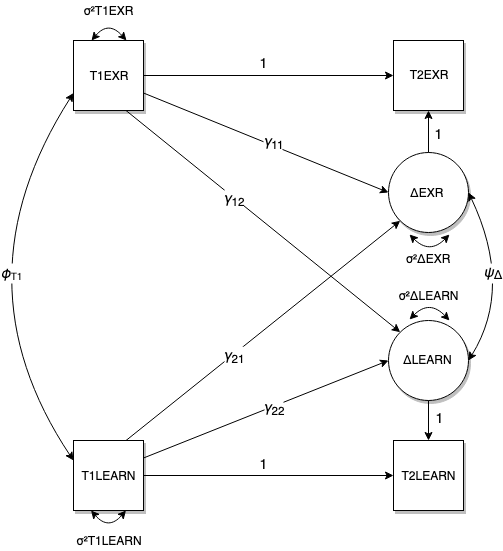
\includegraphics[width=10cm]{Diagram.png}
\caption{Simplified bivariate latent change score model for the effect of exploration and learning at Time 1 on change in exploration and learning from Time 1 to Time 2. Means and item loadings are omitted for visual clarity. Figure adapted from \textcite{Kievit2018}}.
\end{figure}


\begin{figure}[t]
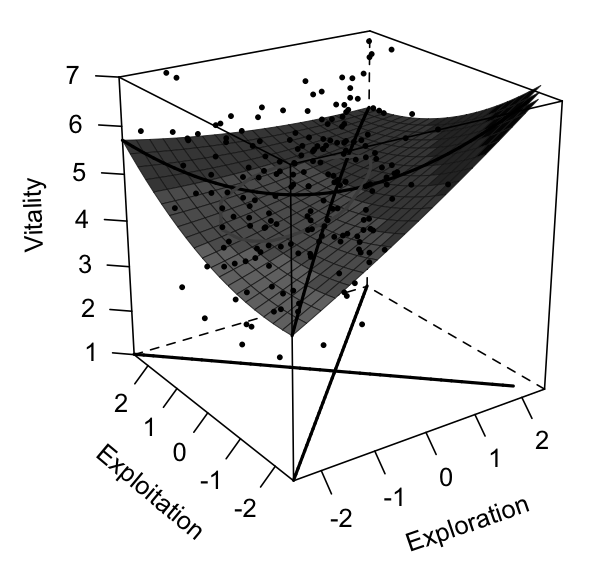
\includegraphics[width=8cm]{Plot.png}
\caption{Response surface plot of the relationships among exploration, exploitation, and vitality at work.}.
\end{figure}

\printbibliography
\end{document}
